Test prints were performed on an unmodified Ultimaker S5 system,
with a standard  \SI{0.4}{\milli\meter} nozzle
and PLA filament
and a layer thickness of $h=\SI{0.1}{\milli\meter}$.
In order to accurately realize a varying bead width we vary the movement speed, while keeping the internal pressure in the system constant.
One approach would be keep the filament inflow $f$ (in \si{\milli\meter\cubed\per\second}) constant by varying movement speed accordingly.
However, that doesn't result in the intended filament outflow variation - see \cref{zero_backpressure}.
We conjecture that the filament outflow is related to the total pressure in the system,
which depends not only on the amount of filament in between the feeder wheel and the nozzle (which we keep constant), 
but also depends on the backpressure that the previous layer exerts on the filament protruding from the nozzle.
We conjecture that the amount of backpressure is monotonically related to the requested line width and compensate for the backpressure using a simple linear model:

\begin{align}
 v(w) &= \frac{f(w)}{h w} \\ 
% f &\sim p \\
% p &= p_\text{in} + p_\text{ext} \\
% p_\text{in} &= C \\
% p_\text{ext} &\sim w \\
% p_\text{ext} &= w / w^* - 1 \\
% f &= f^* - k p_\text{ext} \\
 f(w) &= f_0 - k \left( w / w_0 - 1 \right) \\
 f_0 &= v_0 w_0 h 
% v &= \frac{f^* - k p_\text{ext}}{h w} \\ 
% v &= \frac{v^* w^* h - k (w / w^* - 1)}{h w}
\end{align}
where
$v(w)$ is the movement speed as a function of requested bead width $w$,
$f(w)$ is the filament outflow,
$f_0$ is a constant reference flow
and
$k$ is the amount of backpressure compensation.
Using increments of $0.1$ we established that using a factor of $k=1.1$ yields satisfactory bead width variation for our setup where
$v_0=\SI{30}{\milli\meter\per\second}$, 
$w_0=\SI{0.4}{\milli\meter}$.
See \cref{backpressure}.

\begin{figure}
\centering
\setlength{\figwidth}{0.32\columnwidth}
\setlength{\figheight}{0.5\columnwidth}
\begin{subfigure}[t]{\figwidth}\centering
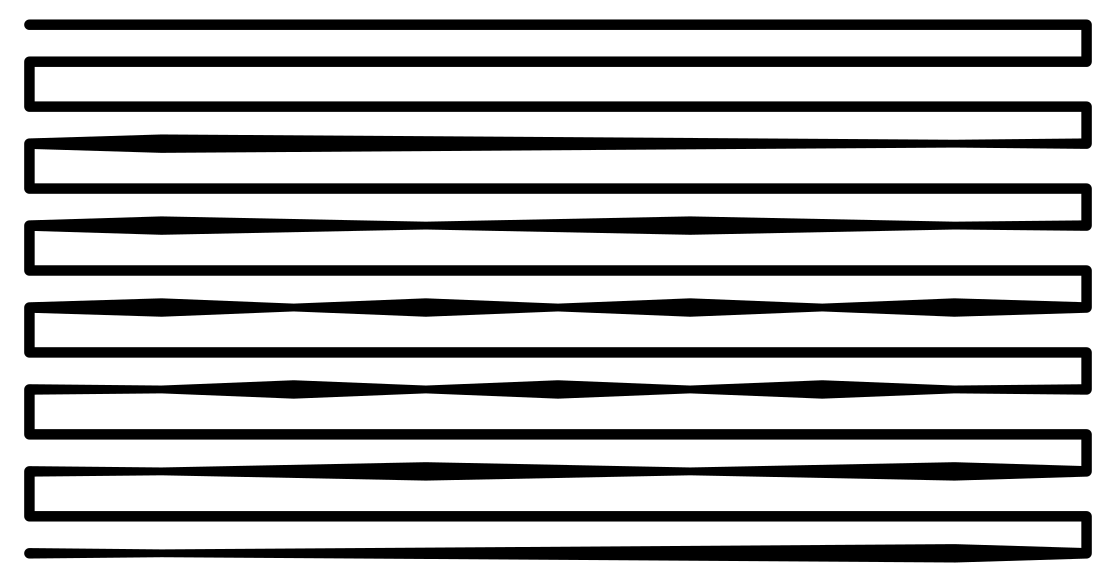
\includegraphics[angle=90,height=\figheight]{sources-validation-backpressure-compensation-target.pdf}
\caption{Target widths}\label{backpressure_target}
\end{subfigure}
\begin{subfigure}[t]{\figwidth}\centering
\includegraphics[angle=90,height=\figheight]{sources-validation-zero-backpressure-compensation.png}
\caption{Constant filament inflow (\si{\milli\meter\cubed\per\second})}\label{zero_backpressure}
\end{subfigure}
\begin{subfigure}[t]{\figwidth}\centering
\includegraphics[angle=90,height=\figheight]{sources-validation-backpressure-compensation.png}
\caption{Backpressure compensation}\label{backpressure}
\end{subfigure}
\caption{
Print results of varying width test on top of a dense white raft.
Trying to reproduce \subref{backpressure_target} without backpressure compensation ($k=0$) yields worse results \subref{zero_backpressure} than with backpressure compensation $k=1.1$ \subref{backpressure}.
}
\label{backpressure_compensation}
\end{figure}


% adapted from 5.5 Discussion on implications
\todo{Reword the following paragraph, which is adapted from 5.5 Discussion on implications.}

Note that the current industry standard in FDM printing employs little to no bead width variation.
\revise{
Properly performing bead width variation calls for adaptations and developments in printers and firmware.
In the beading schemes we set a transition length of $t(n) = w^*$.
That will demand changes in cross-sectional area of the bead up to \SI{200}{\percent} over a small distance that is comparable to the nozzle size, which is challenging for some hardware systems.
Varying the movement speed can be utilized to change the cross-sectional area, 
}{While some software packages generate toolpaths similar to the state-of-the-art,
the naive constant width offset approach is still widely used.
Our backpressure compensation algorithm effectively changes the speed to realize adaptive width,
}
but this approach is limited, since the movement speed is constrained by acceleration considerations near bends in the toolpath~\cite{Ertay2018,Kuipers2018}.
\revise{
Our schemes require a more accurate control of the volumetric flow rate in \si{\milli\meter\cubed\per\second}.
}{}
Using a filament feeder directly mounted on the print head (a.k.a. direct drive) can \revise{control the flow more dynamicaly}{provide more dynamic control over the flow} \revise{then}{than} FDM printers where the material is fed through a Bowden tube from a feeder mounted on the frame.
\revise{
Still direct drive printers require some control system in order to accurately change the volumetric flow rate such as pressure advance algorithms~\cite{tronvoll2019investigating}.
Yet inaccuracies in direct drive systems employing advance algorithms might arise due to the changes in back-pressure required by changing bead size.
We expect that developments in printing hardware and firmware will address these challenges in the future.
}{Direct drive printers can benefit from \emph{pressure advance algorithms} which dynamically change the internal pressure \cite{tronvoll2019investigating},
but presumably backpressure would still be a significant factor one might want to compensate for.
}


\todo{For super small layer heights it might be impossible to reach a bead width range with a factor of $2$.}

Another limiting factor for adopting adaptive bead width is the format of G-code which stores machine instructions.
G-code does not support moves with varying cross-sectional area.
A typical extrusion move \lstinline{G1 X$x$ Y$y$ E$v$} only specifies the total amount of volume $v$ to be extruded in the move, not how that total amount should be distributed along the extrusion move.
A workaround is to approximate a variable width extrusion segment by smaller segments with constant width.
However, this introduces errors nevertheless.
Ideally the G-code language would be expanded in some way to allow for extrusion segments with varying cross-sectional area.
